\section*{The screen is the load-bearing step}

Of the three cleaning levels, only the last produces a fit that is admissible
at all.

Cancellation --- $\sum \beta^2 / h^2$, the ratio that detects effects adding up
through LD rather than to the heritability they are supposed to explain ---
starts at $255$ for LDL and stays there through per-variant filtering, reaching
$271$. Minor allele frequency, imputation quality and a $\chi^2$ cap remove
37{,}000 variants and leave the pathology untouched, because none of them can
see it: each judges a variant on its own. The screen drops a further 42{,}000
and cancellation falls to $0.65$.

\begin{figure}[H]
\centering
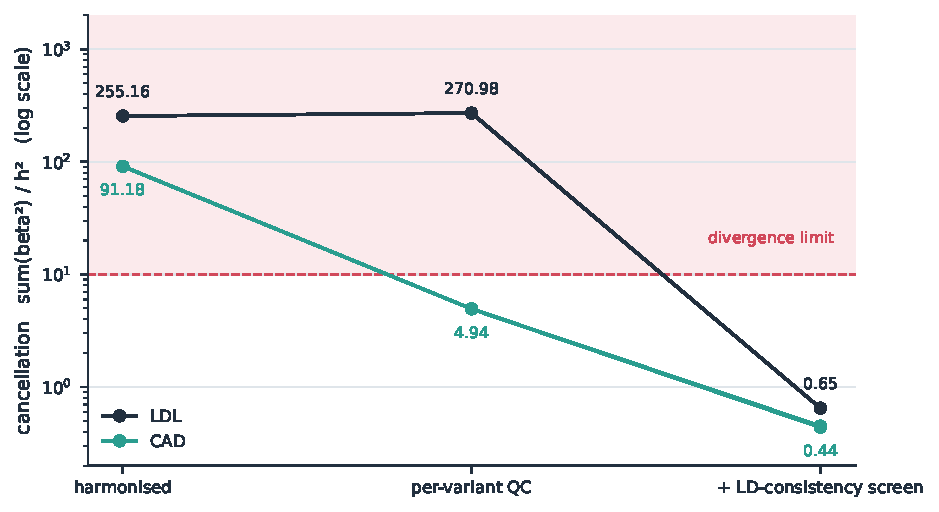
\includegraphics[width=\linewidth]{figures/cancellation.pdf}
\caption{Cancellation by cleaning stage, log scale. Above the limit of $10$ the
sampler is placing large opposing effects on variants in near-perfect LD, and
the heritability it reports is those effects cancelling rather than explaining.
Per-variant filters move LDL the wrong way. CAD crosses the limit at the
per-variant stage but only clears it after the screen. Both platform runs are
drawn; they coincide closely enough to be one line each.}
\end{figure}

Only after the screen do all three divergence diagnostics clear. That is what
makes the third row an estimate and the first two not.

\begin{figure}[H]
\centering
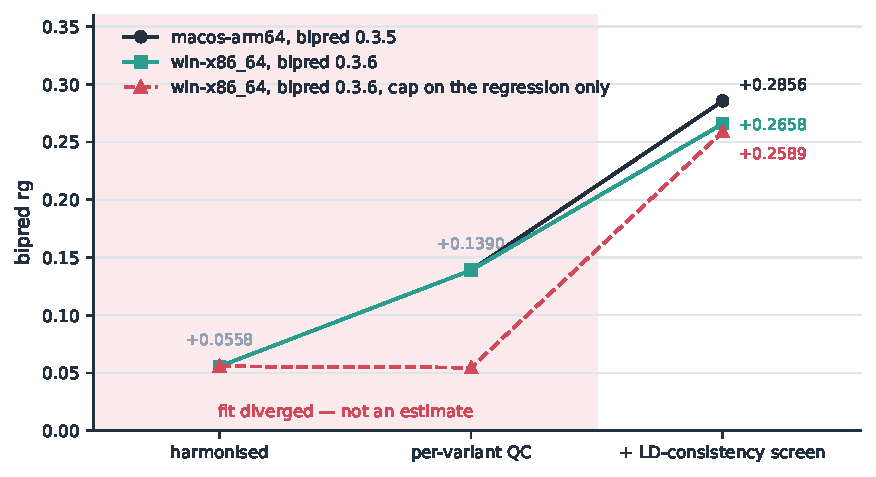
\includegraphics[width=\linewidth]{figures/rg-by-stage.pdf}
\caption{Genetic correlation by cleaning stage. The shaded region marks the
stages where the fit carried a divergence warning: the $+0.0558$ and $+0.139$
plotted there are what a diverged sampler emitted, not estimates of anything,
and the apparent trend across the three points is not a convergence toward a
right answer. The $\sim{+}0.27$ that emerges is a consequence of the fit
becoming valid.}
\end{figure}

Heritability moves with it. LDL's $h^2$ falls from $0.67$ to $0.09$ across the
three stages, which is the same phenomenon read on a different scale: the
$0.67$ was cancellation, not signal.

This is one trait pair. It is why the screen exists and why arm 001 fixes it
on; it does not establish a universal QC rule, and the
$2 \times 2 \times 2$ factorial that would support one is in
\texttt{benchmarks/qc\_factorial.py}.

\subsection*{What the chi-square cap does here: almost nothing}

The third run in \texttt{results/estimates.csv} repeats all three stages with
\texttt{--chi2-cap ldsc}, which holds high-chi-square rows out of the LD Score
regression --- which needs them held out --- while the joint fit keeps every
variant. The dashed line in the figure above is that run.

At the stage that counts it changes nothing. \texttt{rg} moves from $+0.2658$
to $+0.2589$, a shift of $0.0069$. That is smaller than the fit's own iterate
spread at that stage ($0.0148$) and about a third of the $0.0198$ that bipred
0.3.6's mask reseed already moved it. Heritability moves in the fourth decimal,
cancellation stays at $0.7$ and $0.5$, and no diagnostic changes state.

At stage 2 it changes a great deal --- $+0.139$ against $+0.0546$ --- and that
contrast is the informative part. Both of those fits are diverged, so neither
is an estimate of anything. What the pair of numbers shows is that
\textbf{the cap and the screen remove largely the same variants}: the two fit
sets differ by 426 variants before screening and by one afterwards. On this
pair the screen was already doing the cap's work, which is why taking the cap
off changes nothing that survives to the end.

That is a statement about LDL and CAD, not about the filter. They lose 7.6\%
and 0.4\% of their summed chi-square to it. The traits where it removes half
the signal are in the companion study, and this run says nothing about them.
